\subsubsection{\bf Introduction}
The RMSMonitor is a tool to investigate the non-stationary behavior of the input time series $x(t)$ by calculating the band-limited root-mean square(for short RMS) values.

The RMS values, $\rho_{RMS}(t)$, of input time series, $x(t)$, are calculated as 
\begin{align}
	\rho_{RMS}(t) = \sqrt{ \int_{f_1}^{f_2} |\tilde{x}(f)|^2 df } \label{RMS}
\end{align}
where $f_1$ and $f_2$ are the frequency band and $\tilde{x}(f)$ is the input frequency domain signal calculated by FFT as,
\begin{align*}
  \tilde{x}(f) = {\rm FFT}[x(t)].
\end{align*}


\subsubsection{{\bf Function:} rmsMon}
{\tt rmsMon nmon fs ys freq\\}

This function compute the RMS, $\rho_{RMS}(t)$, of the input time series $x(t)$.
The time series $x(t)$ are divided into small chunks. The RMS value is calculated from each chunk. The number of chunks are calculated by $ N_{ys} / {\tt nmon}$, where $N_{ys}$ is the number of samples of input time series.\\
The arguments are:
\begin{itemize}
\item {\tt nmon}: [Input] The number of samples in one chunk.
\item {\tt fs}: [Input] The sampling frequency of input time series.
\item {\tt ys}: [Input] The input time series.
\item {\tt freq}: [Input] The frequency bands [$f_1:f_2$] described in Eq. (\ref{RMS}). 
\item {\tt {RMS}}: [Output] The calculated RMS values. 
\end{itemize}


\subsubsection{{\bf Function:} rmsMonWaveData}
{\tt rmsMonWaveData nmon freq wd\\}

This function compute the RMS, $\rho_{RMS}(t)$, of the input time series $x(t)$.
The difference between {\tt rmsMon} and {\tt rmsMonWaveData} is the type of input time series.
{\tt rmsMonWaveData} uses WaveData type instead of the time series $x(t)$.
The other arguments are same as {\tt rmsMon}.\\
The arguments are:
\begin{itemize}
\item {\tt nmon}: [Input] The number of samples in one chunk.
\item {\tt wd}: [Input] The input data ({\tt WaveData} type).
\item {\tt freq}: [Input] The frequency bands [$f_1:f_2$] described in Eq. (\ref{RMS}). 
\item {\tt {RMS}}: [Output] The calculated RMS values. 
\end{itemize}


\subsubsection{{\bf Example:} studentRayleighMon}
This program calculates the $\rho_{RMS}$ of the input time series.
Examples of RMSMon are described in Fig. \ref{fig:RMS1} and \ref{fig:RMS2}.


\begin{figure}[ht]
  \begin{center}
    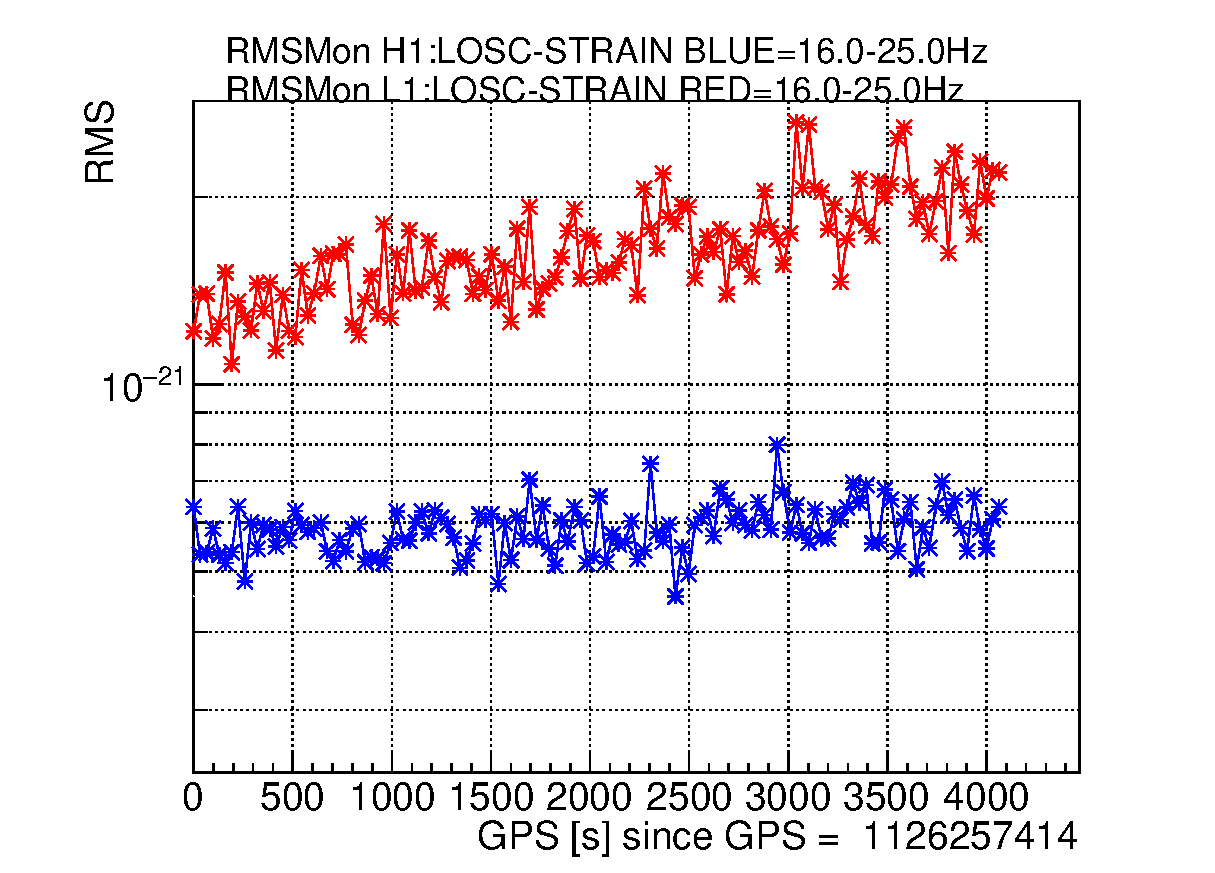
\includegraphics[width=0.9\hsize]{./fig/RMSMon/sample_16-25.eps}
    \caption{Sample plot of RMSMon. The duration of one chunk is 32s. The frequency bands is [16:25]Hz}
     \label{fig:RMS1}
  \end{center}
\end{figure}

\begin{figure}[t]
  \begin{center}
    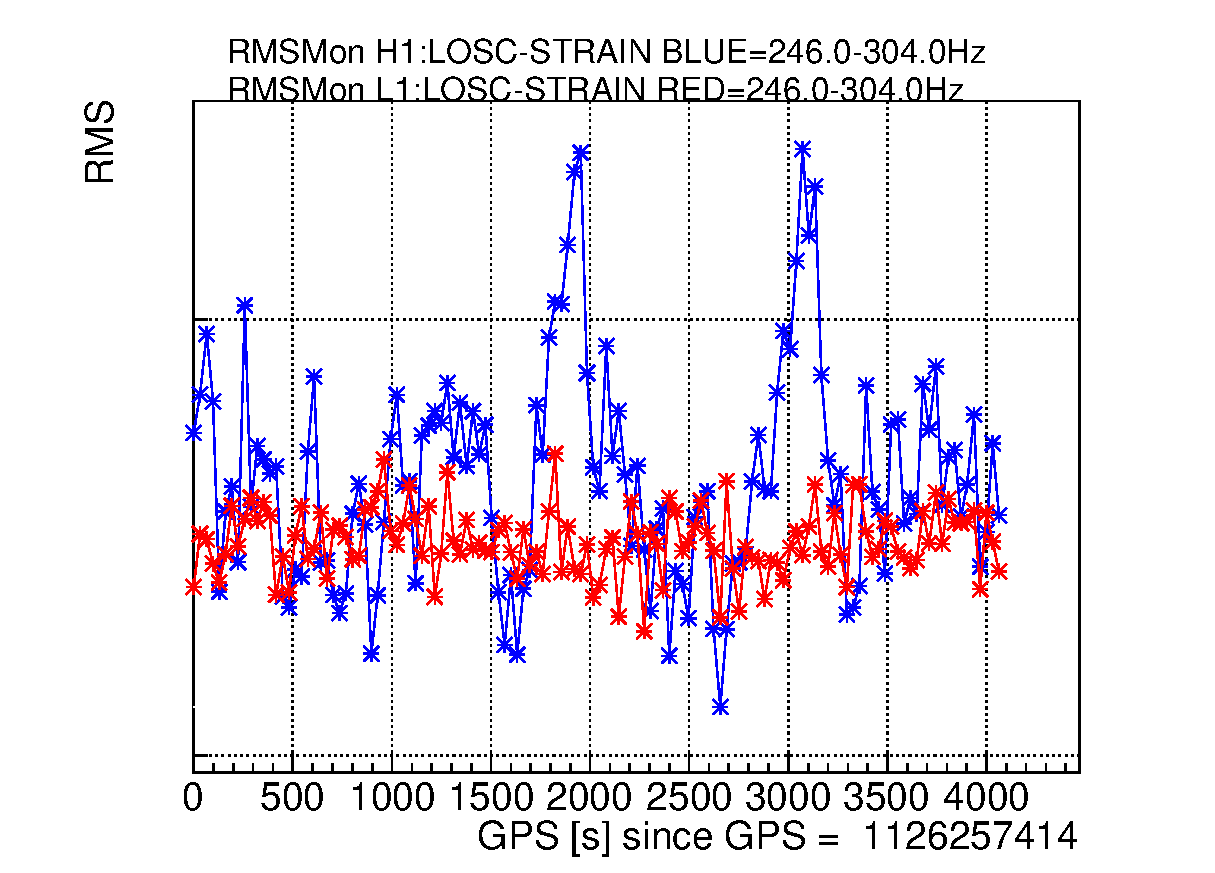
\includegraphics[width=0.9\hsize]{./fig/RMSMon/sample_246-304.eps}
    \caption{Sample plot of RMSMon. The duration of one chunk is 32s. The frequency bands is [246:304]Hz}
     \label{fig:RMS2}
  \end{center}
\end{figure}

{\noindent \small contact person: Hirotaka Yuzurihara (\tt yuzurihara@yukimura.hep.osaka-cu.ac.jp)}

